\section{Auswertung}
\label{sec:Auswertung}

%\subsection{Fehlerrechnung}
\label{sec:Fehlerrechnung}
Für die Fehlerrechnung werden folgende Formeln aus der Vorlesung verwendet.
für den Mittelwert gilt
\begin{equation}
    \overline{x}=\frac{1}{N}\sum_{i=1}^N x_i ß\; \;\text{mit der Anzahl N und den Messwerten x} 
    \label{eqn:Mittelwert}
\end{equation}
Der Fehler für den Mittelwert lässt sich gemäß
\begin{equation}
    \increment \overline{x}=\frac{1}{\sqrt{N}}\sqrt{\frac{1}{N-1}\sum_{i=1}^N(x_i-\overline{x})^2}
    \label{eqn:FehlerMittelwert}
\end{equation}
berechnen.
Wenn im weiteren Verlauf der Berechnung mit der fehlerhaften Größe gerechnet wird, kann der Fehler der folgenden Größe
mittels Gaußscher Fehlerfortpflanzung berechnet werden. Die Formel hierfür ist
\begin{equation}
    \increment f= \sqrt{\sum_{i=1}^N\left(\frac{\partial f}{\partial x_i}\right)^2\cdot(\increment x_i)^2}.
    \label{eqn:GaussMittelwert}
\end{equation}
\subsection{Bestimmung des Schwellenstroms}
\label{sec:Ausw1}
Zur Bestimmung des Schwellenstroms wird wie in \autoref{sec:AufbLasergran} vorgegangen. Dadurch konnte von Schwellenstrom von $34.9\,\unit{\milli \ampere}$ ermittelt werden. Die zugehörigen Bilder hierzu sind \autoref{fig:befTresh} und \autoref{fig:Boom}.

\begin{figure}
    \centering
        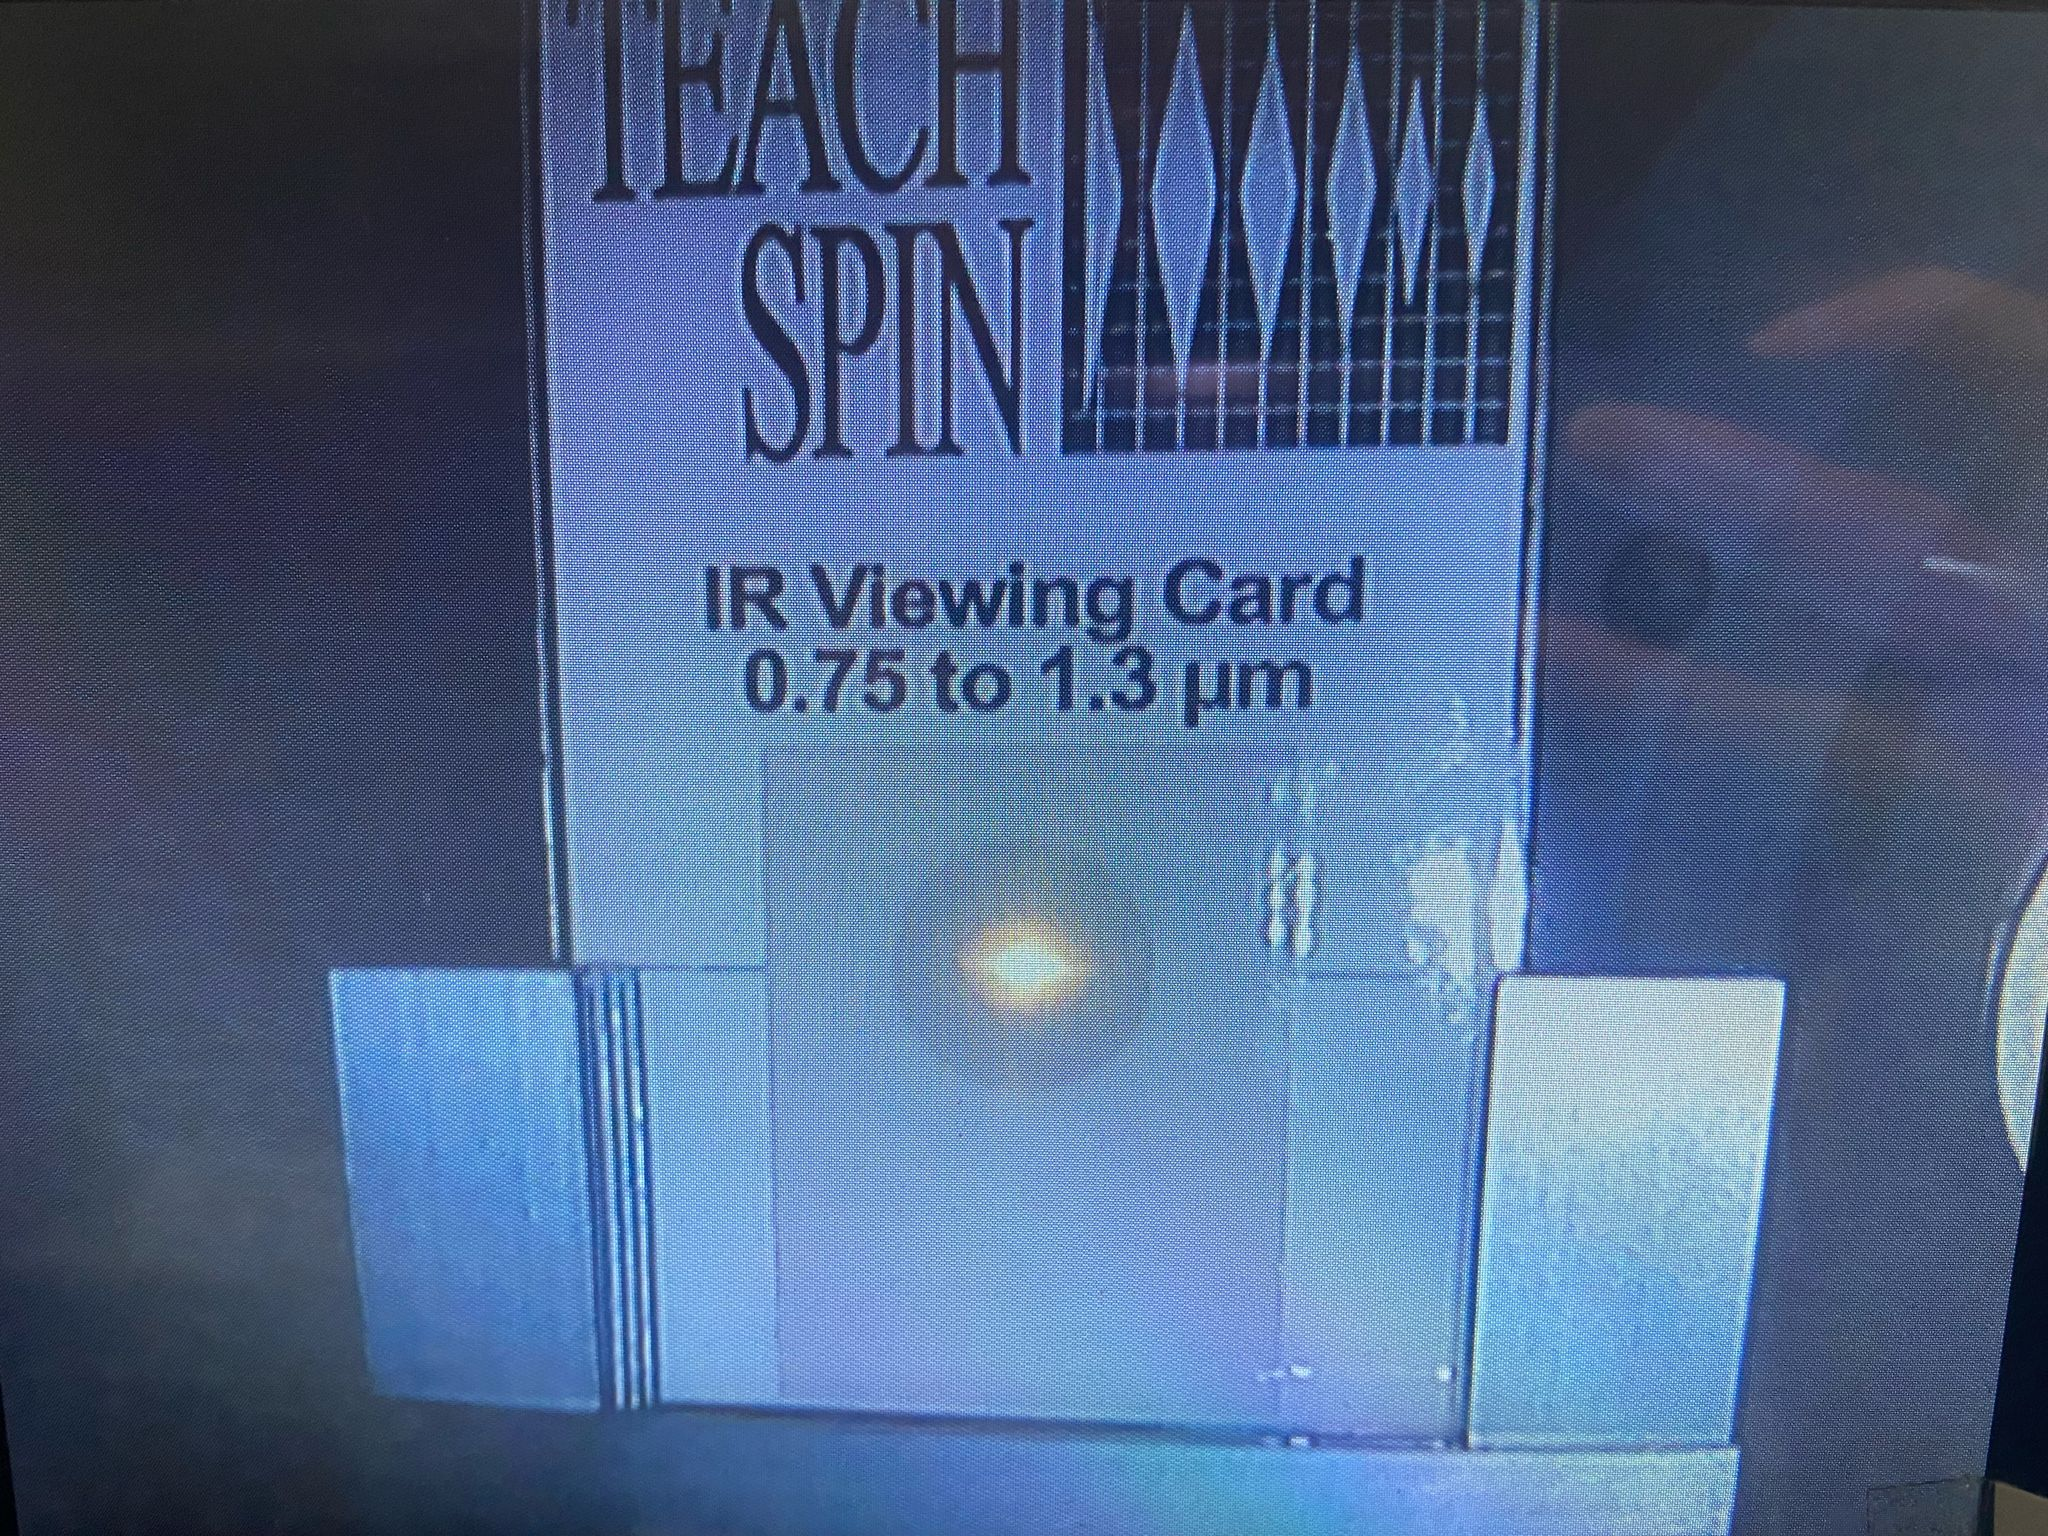
\includegraphics[width=0.8\textwidth]{beforeThreshold.jpeg}
        \caption{Lichtbild unterhalb des Schwellenstroms ($34.1\,\unit{\milli \ampere}$).}
        \label{fig:befTresh} 
\end{figure}
\begin{figure}
    \centering
        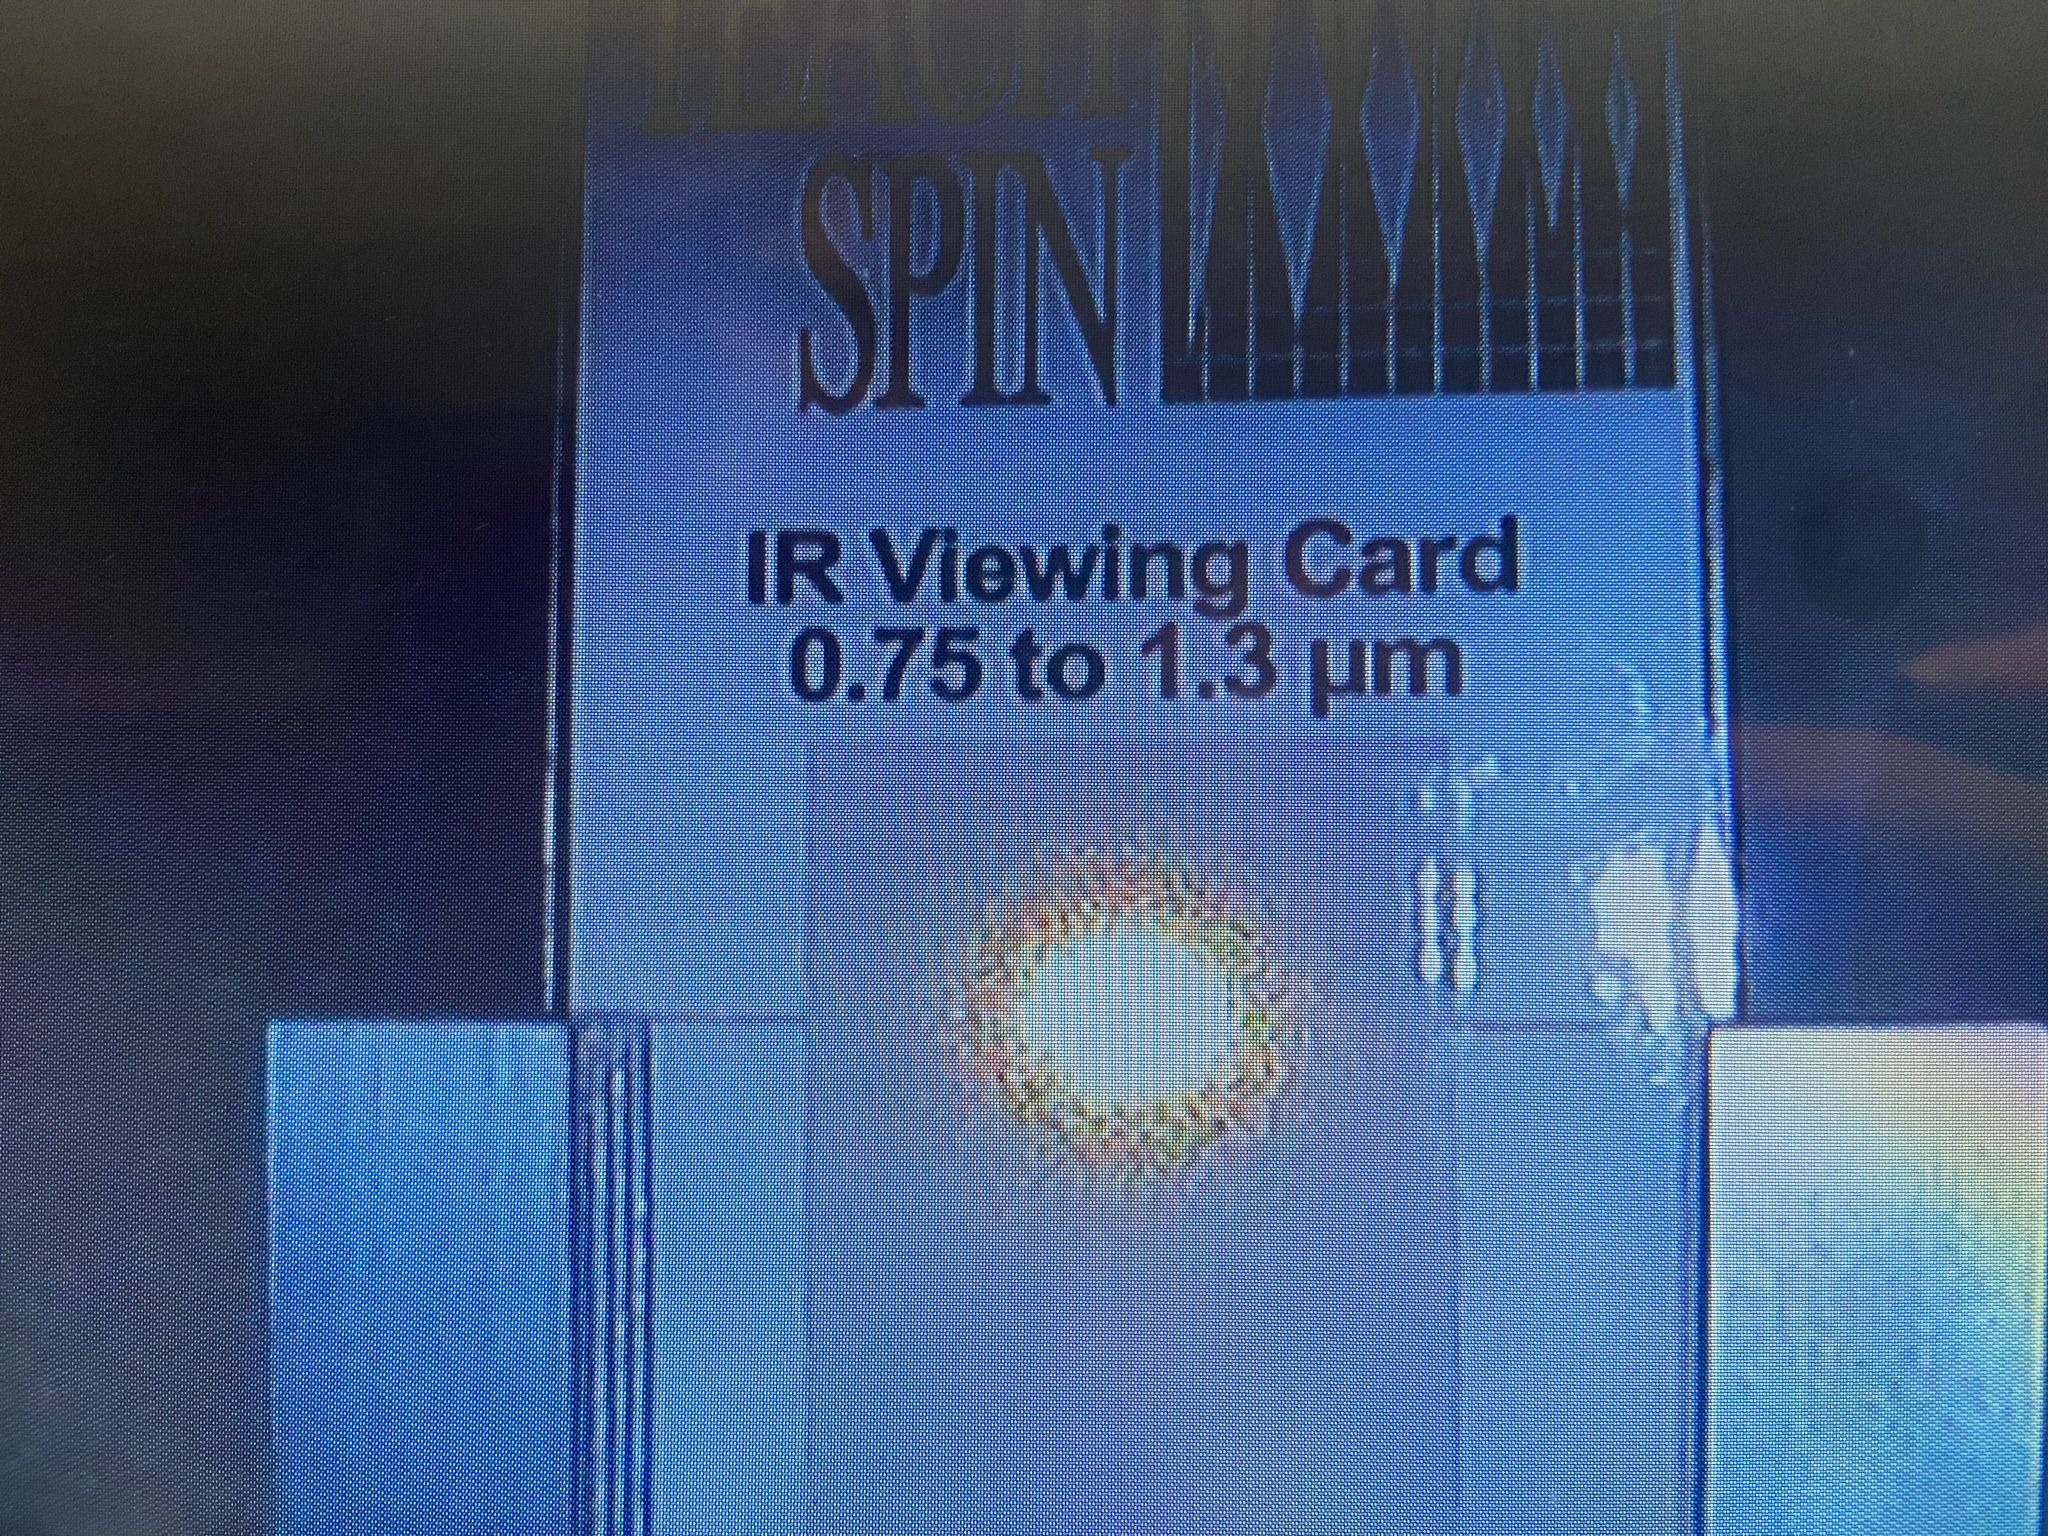
\includegraphics[width=0.8\textwidth]{Lasergranulation.jpeg}
        \caption{Lasergranulation über Schwellenstroms ($36.4\,\unit{\milli \ampere}$).}
        \label{fig:Boom} 
\end{figure}

\subsection{Rubidium-Floureszenz und dessen Spektrum}
\label{sec:Ausw2}
In \autoref{fig:Flour} ist deutlich die Linie der Floureszenz zu erkennen. Das Transmissionsspektrum ist in \autoref{fig:Transmis} als gelbe Linie zu sehen. Hierbei sind die in \autoref{fig:RbSpectrum} gezeigten Übergänge zu sehen.

\begin{figure}
    \centering
        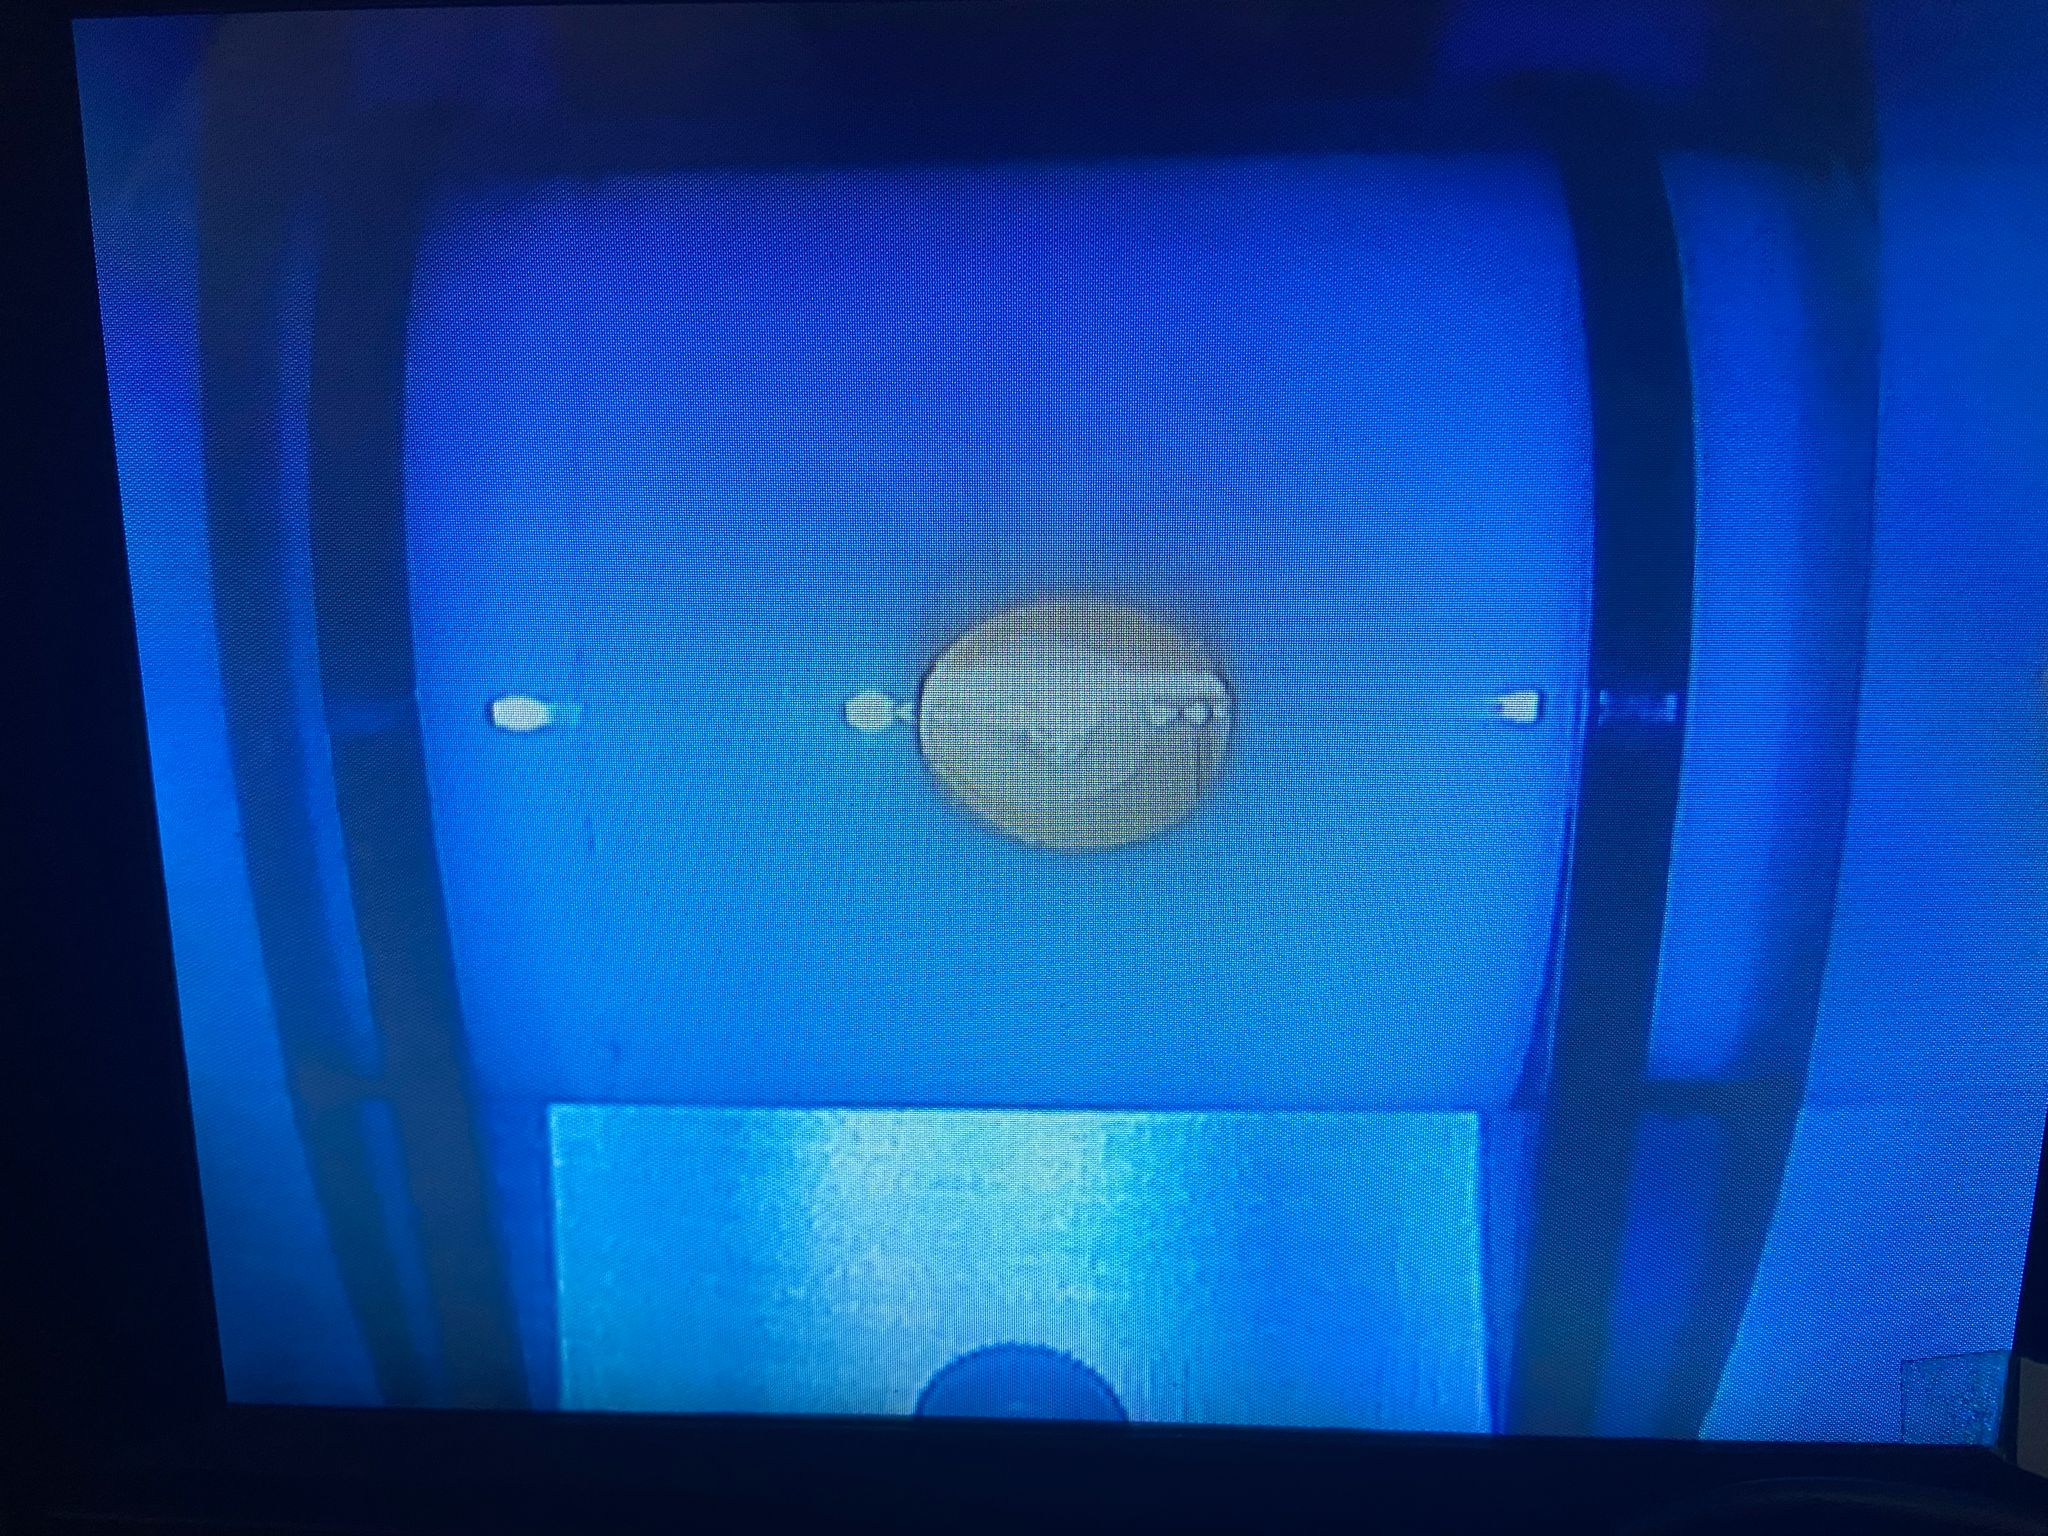
\includegraphics[width=0.8\textwidth]{Luminiszenz.jpeg}
        \caption{Floureszenz des Rubidiums.}
        \label{fig:Flour} 
\end{figure}

\begin{figure}
    \centering
        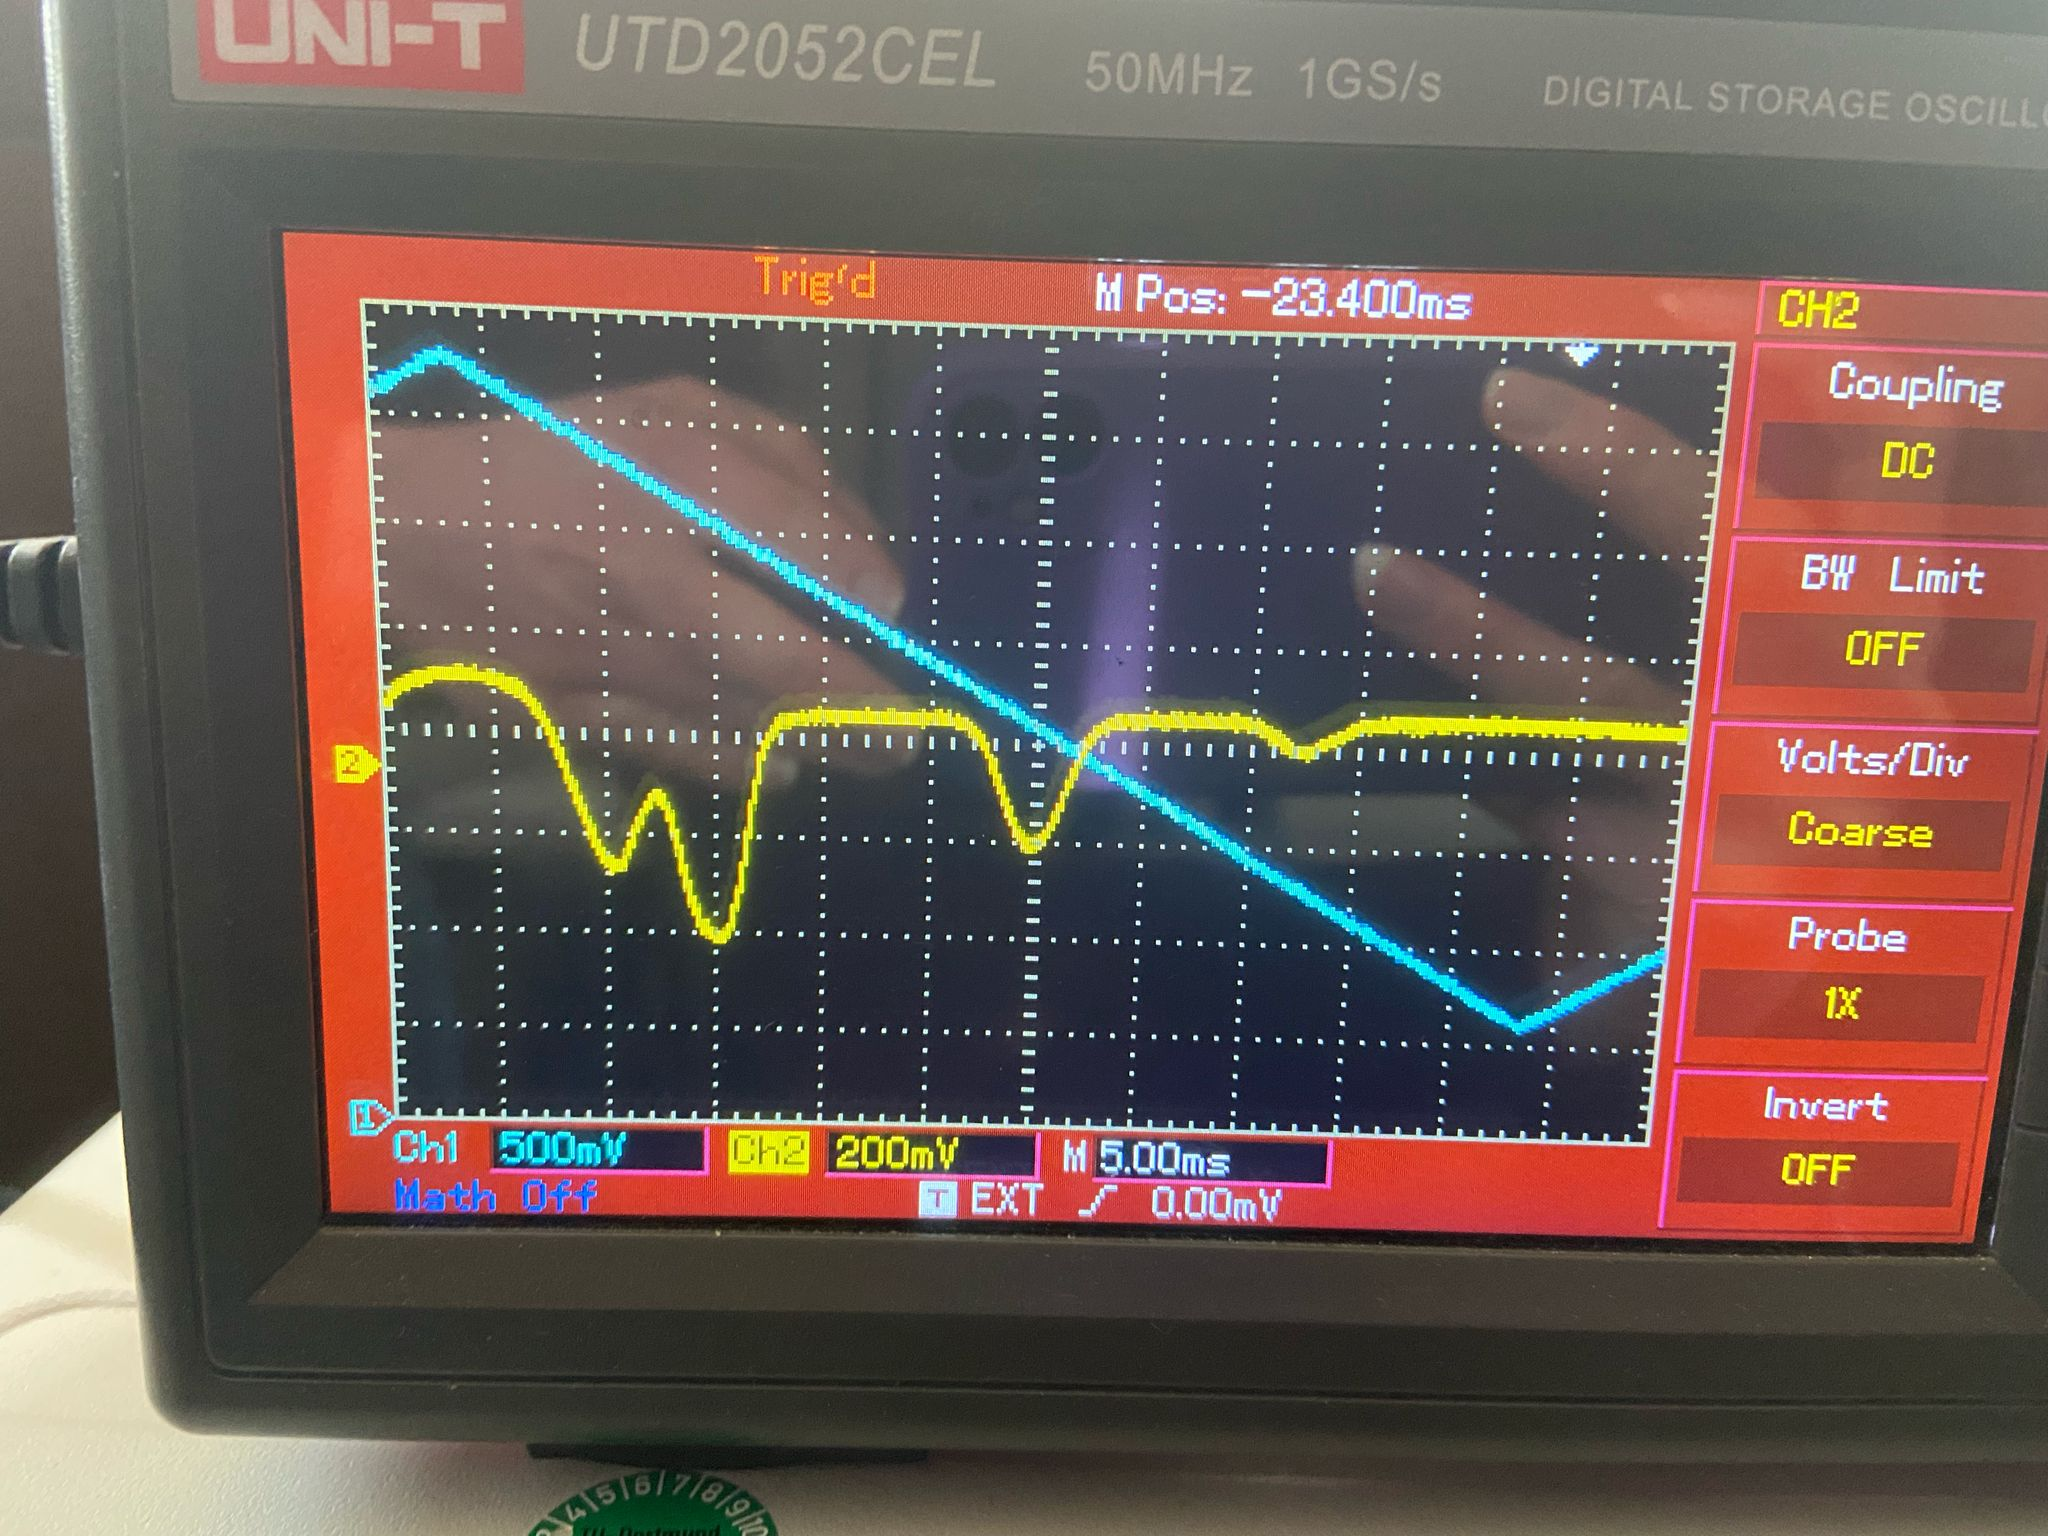
\includegraphics[width=0.8\textwidth]{Spectrum.jpeg}
        \caption{Transmissionspektrum des Rubidiums.}
        \label{fig:Transmis} 
\end{figure}